\section{母模型执行器、跨日续接与结算对照}
\label{app:controllers}

本附录保留原版与未筛选母模型的诊断配置，用于解释规划参考、实时执行和结算响应。最终滚动方案的筛选时点对照及实际收益见正文第\ref{sec:q3_screening_ablation}节。

\subsection{母模型执行器对照：固定合同内层LP}

母模型与最终方案均按当期$a_t,n_t,e_t$执行“富余充电、缺口放电、余缺紧急补购”的规则。以下内层LP与跨日续接对照均基于未启用候选筛选的母模型，用于检验跨时段库存价值估计的作用。

当前时段$t$固定当天剩余常规合同$a_{k|t}$；令当前$\widetilde n_{t|t}=n_t$、$\widetilde p_{t|t}=p_t$，对$k>t$只使用最近合法预报，定义
\begin{equation}
 \begin{cases}
 s_{k|t}=[a_{k|t}-\widetilde n_{k|t}]_+,\\[2pt]
 b_{k|t}=[\widetilde n_{k|t}-a_{k|t}]_+.
 \end{cases}
 \label{eq:v2_surplus_deficit}
\end{equation}
内层优化为
\begin{align}
 \min\quad&\sum_{k=t}^{143}5\widetilde p_{k|t}(b_{k|t}-d_{k|t})
       +\beta_T|e_{144|t}-6000|,\label{eq:v2_inner_objective}\\
 \text{s.t.}\quad&\begin{cases}
 0\le c_{k|t}\le\min\{U,s_{k|t}\},\\
 0\le d_{k|t}\le\min\{U,b_{k|t}\},
 \end{cases}\label{eq:v2_inner_bounds}\\
 &\begin{cases}
 h_{k|t}=b_{k|t}-d_{k|t},\\
 w_{k|t}=s_{k|t}-c_{k|t},\\
 e_{t|t}=e_t^{\rm act},
 \end{cases}
 \label{eq:v2_inner_balance}
\end{align}
同时满足SOC递推、容量和功率约束。$\beta_T$取剩余预测价格中位数，固定常规合同费作为常数略去。只执行第一步储能动作，下一时段根据新实测量重算。

约束\eqref{eq:v2_inner_bounds}以常规供电富余充电，紧急购电仅补负载缺口；富余与缺口互斥，故充放电互斥自动成立。LP可在预测后续缺口更昂贵时保留库存。行为核验中，电池可输出1 kWh，两段合同均为0、需求均为1 kWh、电价分别为1与2元/kWh，关闭终端罚项：规则先放电再付10元补购，LP先付5元补购再放电，程序重现了该差异。

\subsection{母模型执行器对照：跨日预报的续接价值}

6、12、18时的24小时预报分别覆盖次日最初6、12、18小时，即$m=36,72,108$段；零时取$m=0$。跨日候选扩展内层价值估计，次日光伏采用已发布预报，负荷由当日之前已完成的历史日外推。

当$m>0$时，把固定日末罚项替换为
\begin{equation}
 \widehat V_D(e_{144})=\min_{z,c',d',e'}
 \left\{\sum_{j=0}^{m-1}\widehat p'_jz_j+\beta_T|e'_m-6000|\right\},
 \label{eq:v2_continuation}
\end{equation}
续接段遵循与当天一致的储能递推及物理界：
\[
 \begin{cases}
 z_j+d'_j-c'_j\ge\widehat n'_j,\\
 e'_{j+1}=e'_j+\eta_cc'_j-d'_j/\eta_d,\\
 E_{\min}\le e'_{j+1}\le E_{\max},\\
 0\le c'_j,d'_j\le U,\qquad z_j\ge0,\\
 e'_0=e_{144},
 \end{cases}
 \qquad j=0,\ldots,m-1.
\]
$\beta_T$仍由当天剩余预测价格确定。$z_j$等次日变量仅用于估计库存续接价值，正式采购在次日零时确定，实际账单按当天执行量结算。

\subsection{同计划回放：规划与控制的偏差}

本节分别诊断原版12场景配置与未筛选的28场景母模型。原版采用12代表场景、自适应风险基数0.1和备用系数1；重解全年3650个外层决策点，执行区间的重建购电量与保存结果一致。固定计划、初态与历史场景，定义
\begin{equation}
 \Delta_{\rm exec}=\sum_s\pi_s\left(C_s^{\rm replay}-C_s^{\rm plan}\right).
 \label{eq:v2_execution_gap}
\end{equation}
两种费用均为常规采购、调整与紧急采购三项之和。表\ref{tab:v2_execution_gap}中，原版问题二、三、四日前、四滚动在2--12月的平均偏差依次为$-986.50$、$-569.90$、$-1068.47$、$-582.32$元。

\begin{table}[htbp]\centering\small
\caption{原版同计划、同初态、同场景的规划与执行偏差}
\label{tab:v2_execution_gap}
\begin{tabularx}{\linewidth}{LRRRR}\toprule
问题 & 决策点数 & 平均$\Delta_{\rm exec}$/元 & 负偏差比例 & SOC均方根偏差/kWh\\\midrule
问题2 & 334 & -986.50 & 97.90\% & 1319.72\\
问题3 & 1336 & -569.90 & 94.24\% & 994.32\\
问题4-2 & 334 & -1068.47 & 99.40\% & 1350.69\\
问题4-3 & 1336 & -582.32 & 93.94\% & 1048.30\\
\bottomrule\end{tabularx}
\par\smallskip\parbox{\linewidth}{\footnotesize 各决策点先按场景概率加权，再取决策点均值；费用仅含实际结算项目。}
\end{table}


参考储能在场景间共享，实际规则随当前观测改变动作，由此产生双向费用偏差。各剩余日窗口相互重叠，按决策点报告均值。图\ref{fig:q3-execution-band}选取原版问题三正偏差最大的2025年2月9日零时决策，展示同一合同的12场景回放。

\begin{figure}[htbp]\centering
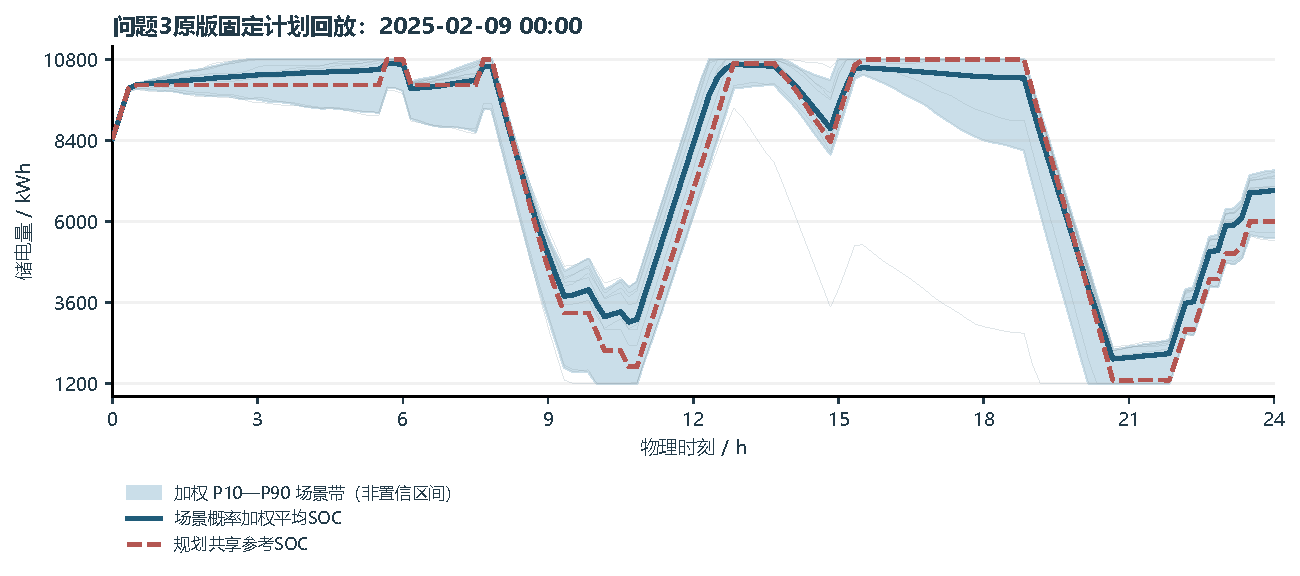
\includegraphics[width=0.95\linewidth]{figures/results/q3_execution_band.pdf}
\caption{原版问题三2025年2月9日零时的12场景规则回放。虚线为共享参考SOC，实线为概率加权均值，细灰线为个体轨迹，阴影为各时刻P10--P90加权经验分位带。}
\label{fig:q3-execution-band}
\end{figure}

在未筛选的28场景母模型上，固定4个指定日、4个外层时点的合同、实际初态与历史场景，对规则和内层LP各回放448条轨迹。每步揭示当步场景净需求和价格，后续沿用决策时点的点预测与合同，以隔离同一计划下更换执行器的影响。

\begin{table}[htbp]\centering\small
\caption{未筛选母模型计划下两种执行器的回放诊断}
\label{tab:v2_inner_gap}
\begin{tabularx}{\linewidth}{LRR}\toprule
指标 & 规则执行 & 内层LP\\\midrule
有符号期望费用偏差/元 & -655.33 & -513.41\\
场景费用绝对偏差的期望/元 & 697.25 & 605.16\\
SOC均方根偏差/kWh & 1056.40 & 869.79\\
\bottomrule\end{tabularx}
\par\smallskip\parbox{\linewidth}{\footnotesize 四个指定日、四个时点共16个决策点，每点28场景。先计算场景概率加权指标，再对决策点等权平均；两种执行器固定相同购电合同和初态，仅逐步揭示当前场景值。}
\end{table}


平均SOC均方根偏差由1056.40降至869.79 kWh，场景费用绝对偏差的期望由697.25降至605.16元，但LP每个决策点的平均回放账单增加141.92元。16点中10点的绝对期望费用偏差减小，仅1点回放费用更低。轨迹贴合度与经济性表现分离，支持直接按固定执行器回放账单筛选采购。

\subsection{母模型内层LP与跨日续接的全年检验}

本节各组均未启用候选筛选，保持原有执行器对照配置。

\begin{table}[htbp]\centering\small
\caption{问题3母模型的执行控制与跨日续接对照}
\label{tab:v2_controllers}
\begin{tabularx}{\linewidth}{LRRRR}\toprule
策略 & 总费/万元 & 紧急量/kWh & 日费CVaR95/元 & 末库存/kWh\\\midrule
规则执行（母模型） & 1397.58 & 12647.76 & 65518.79 & 6240.32\\
剩余日储能LP & 1421.32 & 23825.27 & 66397.37 & 5934.55\\
储能LP+跨日价值 & 1405.26 & 22407.53 & 66033.05 & 6240.32\\
\bottomrule\end{tabularx}
\par\smallskip\parbox{\linewidth}{\footnotesize 未启用候选筛选的母模型对照；各组沿用原实验配置，覆盖334天并连续推进状态。}
\end{table}


在334天闭环中，将母模型规则执行器换成剩余日LP后，费用为14213193.28元，增加237382.42元，紧急量增至23825.27 kWh。

相同LP加入合法跨日信息后，费用降至14052638.61元，减少160554.67元，紧急量减少1417.74 kWh，年末库存增加305.77 kWh，费用仍比规则母模型高76827.75元。各执行器沿用一月冻结配置，采购筛选的时点选型见第\ref{sec:q3_screening_ablation}节。

\subsection{退款口径的独立敏感性}

固定未筛选母模型的预测、场景、执行器与初态，仅切换退款解释后重算。表\ref{tab:v2_settlement}以不退款母模型13975810.86元为基线，衡量结算规则及相应采购响应的影响。

\begin{table}[htbp]\centering\small
\caption{问题3母模型的结算解释敏感性}
\label{tab:v2_settlement}
\begin{tabularx}{\linewidth}{LRRRR}\toprule
策略 & 总费/万元 & 紧急量/kWh & 日费CVaR95/元 & 末库存/kWh\\\midrule
主口径：不退款 & 1397.58 & 12647.76 & 65518.79 & 6240.32\\
取消部分退款 & 1365.55 & 12871.85 & 64278.33 & 6240.32\\
\bottomrule\end{tabularx}
\par\smallskip\parbox{\linewidth}{\footnotesize 未启用候选筛选的母模型对照；各组沿用原实验配置，覆盖334天并连续推进状态。}
\end{table}


退款解释费用13655463.35元，减少320347.51元，累计下调1096916.99 kWh，净调整费用为$-113349.02$元。两组年末库存相同；退款改变取消采购的边际费用，使下调成为有效决策。


\FloatBarrier
